
Virtual reality is a technology which is often regarded as a natural extension to 3D computer graphics with advanced input and output devices \citep{Jayaram1997}. Ryan (2001) defined it as an “interactive, immersive experience generated by a computer” \citep{Ryan2001}. And according to G.C. Burdea and Coiffet (2017) “it is a generated computer graphics used to create a realistic-looking world that responds to the user’s input (gestures, verbal commands, etc.)” \citep{burdea2017virtual}. Virtual reality places the users inside the experience instead of viewing a screen in front of them, the users will be immersed inside a 3D world. As shown in Figure \ref{fig:3I} Three elements are needed to construct a virtual reality situation: immersion, interaction, and imagination. They are called the “3I’s” of virtual reality \citep{Hu2016}.


\begin{wrapfigure}{r}{0.30\textwidth} %this figure will be at the left
    \centering
    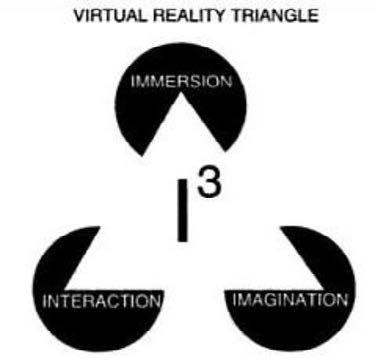
\includegraphics[width=0.30\textwidth]{3I}
    \caption{The 3I's of Virtual Reality - © 2003 by John Wiley \& Sons Inc. All rights
reserved}
    \label{fig:3I}
\end{wrapfigure}

1. \textbf{Immersion:} it is the virtual reality situation where the user feels personally inside the
scene and immerse inside the simulated virtual world.



2. \textbf{Interaction:} The interactive feedback between the user
and the virtual environment. Since it is a man-machine
interface, the system should promptly respond to the
user’s actions.


3. \textbf{Imagination:} The scene design and the construction of
the environment formulated with imagination for a
better user simulated experience.



\section{Political History}


 Palestine, a country that is known by living in political conflict for decades. Palestine was under the British mandate from 1923 to 1948. According to Sa’di \& Abu-Lughod
(2007) “on the last day of the mandate, the creation of the state of Israel was proclaimed,
and the 1948 Arab-Israeli war began” \citep{Sadi2007}. 

\begin{wrapfigure}{r}{0.20\textwidth} %this figure will be at the left
    \centering
    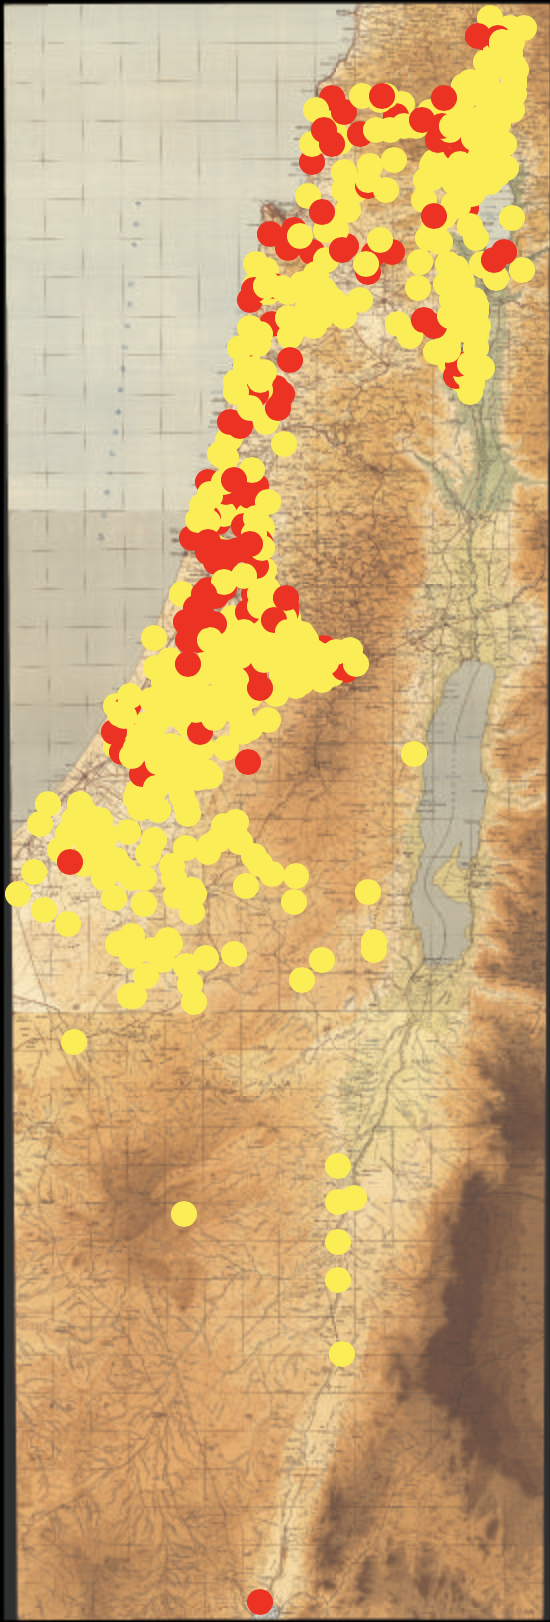
\includegraphics[width=0.20\textwidth]{d_villages}
    \caption{Demolished and depopulated villages - Palestine Open Maps, © 2018  Visualizing Palestine }
    \label{fig:map}
\end{wrapfigure}



The 1948 war that led to the creation of the State of Israel over Palestine also resulted in the devastation of the Palestinian society \citep{Sadi2007}. The day that Israel was created over Palestine, for Palestinians it was a catastrophe (“Nakba” in Arabic). At least 80\% of the Palestinians who lived in the major part of Palestine upon which Israel was established – more than 77\% of Palestine’s territory – became refugees. “The lives of the Palestinians at the individual,
community, and national level were dramatically and irreversibly changed” \citep{Sadi2007}.








The “Nakba” a massive number of Palestinians were deported outside of Palestine. “Of the
1,400,000 Palestinians in the country prior to the Nakba, just 150,000 individuals were listed
as being present during the first census carried out by the new Israeli state” \citep{Sanbar2007}.
According to Falah (1996) “Some of the Israeli military code names of their operations was
Matate (Broom), and Bi’ur Chametz (Passover Cleanup) – suggest that the war involved an
aspect of ethnic cleansing” \citep{Falah1996}\citep{Pappe2006}. The Israeli forces demolished and depopulated 531
Palestinian villages during the 1948 war, as shown in figure \ref{fig:map} the red dots represent the demolished villages, and the yellow dots represent the depopulated villages. According to the \acrshort{unrwa} in January 2015 registered
Palestinian refugees reached more than 5 million, divided between, The West Bank, Gaza
Strip, Syria, Lebanon, and Jordan \citep{DajaniDaoudi2011}. 

Since 1948 the Palestinian refugees are not allowed to return to Palestine, and not even for a visit. Due to the idea of the return of significant numbers of Palestinians to their villages and towns, or indeed to any part of Palestine, touches on deep-seated fears among Israelis regarding the legitimacy and permanence of the entire Zionist enterprise, as well as the Arab-Jewish demographic balance within Palestine \citep{Khalidi2016}. According to Pappé (2006), the Zionist organization and the Hebrew University mapped and made a detailed registry of all the Arab villages \citep{Pappe2006}.



The project of mapping the whole villages details turned out to be a "national Project" and it was called "The village files"\citep{Pappe2006}. In the late 1940's the "archive" was almost complete and the information became more explicitly military orientated \citep{Pappe2006}. In 2018 the Israeli national archive was published online, but after a time of research through the archive in English and in Hebrew, those maps and the detailed information about the villages were not openly published. according to Shezaf (2019), the Israeli defense minitsry secretive security department (Malmab) is responsible for concealing hundreds of documents as a part of a systematic effort to hide evidence of the Nakba.

%The website of the Israeli national archive, gave a form to fill explaining the reasons that the user needs to access such a data, without giving a clear answer if the user will get access to it. 
\section{Cultrual Identity}

\section{Al-Ghabisiyya Village}

Al-Ghabisiyya is located north east acre in distance of 11.5 km. The village stood on a rocky hill that jutted up from the plain of Acre. Judging from the many caves that were used as burial places, the area probably had been a large Canaanite town.
Al-Ghabisiyya was populated by 690 inhabitants, in 1931 it had 125 houses. The village was built in the late nineteenth century, it was inhabited by 150 residents back then\citep{Khalidi1992}.
\subsection{Al-Ghabisiyya before 1948}

 Al-Ghabisiyya was surrounded by a variety of trees like, olives, fig, and pomegranate. The village was near another two Villages Shaykh Dannun and Shaykh Dawud. Shaykh Dawud and Shaykh Dannun were overlapped at points, but Al Ghabisiyya was about 500m away from them. The entire population of these villages was Muslim. 

Al-Ghabisiyya had a school that was built by Ottomans in 1886. The village houses were built of reinforced concrete or, in some cases, stone held together with a mortar of mud or cement. The economy of the village was based on livestock raising and agriculture, grains and vegetables were the chief crops. the villagers also grow olives, which they processed on two animal-drawn presses, one in Al-Ghabissya and one in Shaykh Dawud.

In 1944/45 a total of 6633 dunums of the lands of the three villages was allocated to cereals, 1371 dunums were irrigated or used for orchards. In the same year 300 dunums in Al-Ghabisyya were devoted to olive trees\citep{Khalidi1992}.

\subsection{Occupation and Depopulation}

Al-Ghabisiyya fell at the end of operation Ben-Ami, the Haganah's invasion of the northwest corner of Palestine. The operation, which began 13-14 May 1948, was the last major Haganah offensive before the end of the British Mandate in Palestine. It was designed to capture all the coastal villages from Acre northwards to the Lebanese border\citep{Khalidi1992}.

In the words of Israeli historian Benny Morris, this was "in line with Plan D[alet]'s provision for securing blocks of Jewish settlement even outside the partition plan borders."\citep{Morris2004}

The Carmeli Brigade which carried out the operation, was given the order on 19 May 1948, "to attack in order to conquer, to kill among men, to destroy and burn villages of Al-Kabri, Umm al Faraj and Al-Nahr"\citep{Morris2004}. Al-Kabri was occupied the following night, on 20-21 May, as part of the second stage of operation Ben-Ami. Along with a series of villages in western Galilee, north of Acre, Al-Nahr was captured 20-21 May 1948, during this second phase of the opertation. Units of the Carmeli Brigade attacked Al-Ghabisiyya it was the last village taken on 20-21 May 1948. Al-Ghabisiyya surrendered formally and that some of its population were expelled sometime during the following days or weeks\citep{Morris2004}.

The attack was waged from two directions, the north and southeast. The occupying forces captured a house in the southernmost corner of the village and proceeded to shell the village from the house, killing and injuring many of the villagers while they were fleeing. Others had been evacuated earlier, due to the fall of Acre. The village militia decided to not confront the Zionist forces because they were too few (around twenty) and very poorly armed. Most of those who were driven out remained in other villages in Galilee until the whole region fell at the end of October 1948, after that they were displaced to Lebanon\citep{Khalidi1992}.

Some inhabitants remained in Al-Ghabisiyya until Febrauary 1949. During that month, there was a second explsionm this time by the Military Government, on grounds of "security and order". it is not clear where they expelled villagers were taken\citep{Morris2004}.

After Al-Ghabisiyya and its two neighboring villages of Shaykh Dannun and Shaykh Dawud were evacuated, the Israeli government permitted some of the inhabitants of the latter two villages to return to their homes. Those who had not sought refuge in Lebanon came back and were joined by a few families from Al-Ghabisiyya, Al-Nahr, Al-Tall, Umm Al-Faraj, 'Amqa, and Kuwaykat. The two small villages of Shaykh Dannun and Shaykh Dawud were merged to form a joint village called Shaykh Dannun, in 1973 it had a population of about 1000. The Village of Al-Ghabisiyya was not repopulated \citep{Khalidi1992}.  

\subsection{The Village Today}

The only landmark that remains is the mosque, a doomed, stone structure, with arched doors and windows and decorative arches in the interior. It is deserted, the cement plaster on the doom is peeling off, and wild shrubs cover the rest of the roof. The debris of houses, terraces, and the village cemetery can be seen among a thick forest of cypress trees that was planted on the village site and part of the land. Cactuses also grow on the site. The settlement of Netiv ha-Shayyara that was established by Iraqi Jewish immigrants in 1950, uses the adjacent non-forested land for agriculture.    

\section{The YALLAH! Hackathon}

\acrshort{yallah!} Is a student’s exchange research program between the University of Siegen in
Germany and Birzeit University in Palestine funded by the DAAD. The program was
constructed for a collaboration between students to create social innovation projects.
In \acrshort{yallah!} 2018 there were three different projects Mobile Makerspace, VR Experience and
\acrshort{yallah!} Computer Club. The \acrshort{yallah!} program is divided into three phases: The preparation
phase (boot camp), a research phase in Germany, and an implementation phase in Palestine.
The \acrshort{yallah!} Hackathon preparation phase
The participants of \acrshort{yallah!} learned about some research methods and how to apply them in
the projects through a boot camp week. During the boot camp, the teams took their first
steps in the projects by planning the research track, setting a research question, and building
a strategy to achieve their goals.
The Palestinian and the German students attended the boot camp separately, therefore the
boot camp took a place once in Germany and another time in Palestine. The purpose of the
boot camp was to introduce and train the participants on the research methods (such as how
to make interviews, how to take field notes, and how to observe while working in the field).
The students split up into 3 groups each group studied one method through literature and
then presented it to the other participants. By the end of the presentation, the students
discussed the method together and practiced it inside the group. The boot camp was very
good practice for the methods and emphasized the research skills of the participants. At the
boot camp in Germany, the Virtual reality project students made their first test in filming with
a 360o camera, they used the Samsung Gear 360 camera to record part of the boot camp
sessions in a purpose to use it later in the project as a testing video. Due to the average video
quality of the Samsung Gear 360 camera, the VR students added a task to their list that is to
find a 360o camera with better quality. The students also discussed the interesting spots in
Palestine related to the historical and religious places mentioned in biblical stories.
The \acrshort{yallah!} Hackathon research phase
The Palestinian students visited Germany for the research phase. The Palestinian and the
German exchange students met in Siegen, Germany for the first time. The students gathered
on the first day and had an introduction from the supervisors about the whole \acrshort{yallah!}
program in general and the research phase in Germany. After the introduction on the first
day, the teams of each project gathered and discussed their plans for the research and the
implementation phases. The VR team members discussed the kind of methods to be used in
the research, the team decided on Interviews and Thinking Aloud as methods for collecting
data from random people and from Palestinians who live in Germany. Therefore, there were
multiple tasks needed to be done by the team to start working with those methods. The VR
team split the tasks among the members: creating the interview questions guideline,
documentation, building a prototype, and logistics, for instance, to create a contact list of
interesting people to contact and have an interview with them.
After one month after the end of the research phase, the VR team had their second gathering
in Palestine to start the implementation phase. The implementation phase contained a lot of
filming in different places in Palestine. Depending on the research results and the discussion
with the team members, they created an organized plan for visiting different places in
Palestine and capturing the area using the camera. The plan included the main cities of
Palestine, famous touristic sightseeing locations and religious places since people showed
high interest to see those spots. Therefore, the team recorded in Jerusalem, Jaffa, Haifa, Akka
(Acre), Ramallah, Nablus, Jericho, Hebron, and Bethlehem.
\subsection{VR Application development}